\chapter{Экспериментальная часть}

\section{Технические характеристики}

Технические характеристики устройства, на котором выполнялось тестирование, следующие.

\begin{itemize}
	\item Операционная система Fedora linux 36 \cite{linux}.
	\item Оперативная память: 16 Гб.
	\item Процессор: AMD Ryzen 7 5800U with Radeon Graphics, 1901 МГц, ядер: 8, логических процессоров: 16.
\end{itemize}

\section{Демонстрация работы программы}

На рисунке \ref{img:example} представлен результат работы программы, если на вход поступили строчки \textit{wood} и \textit{blood}.

\begin{table}[h!]
	\centering
	\begin{tabular}{p{1\linewidth}}
		\centering
		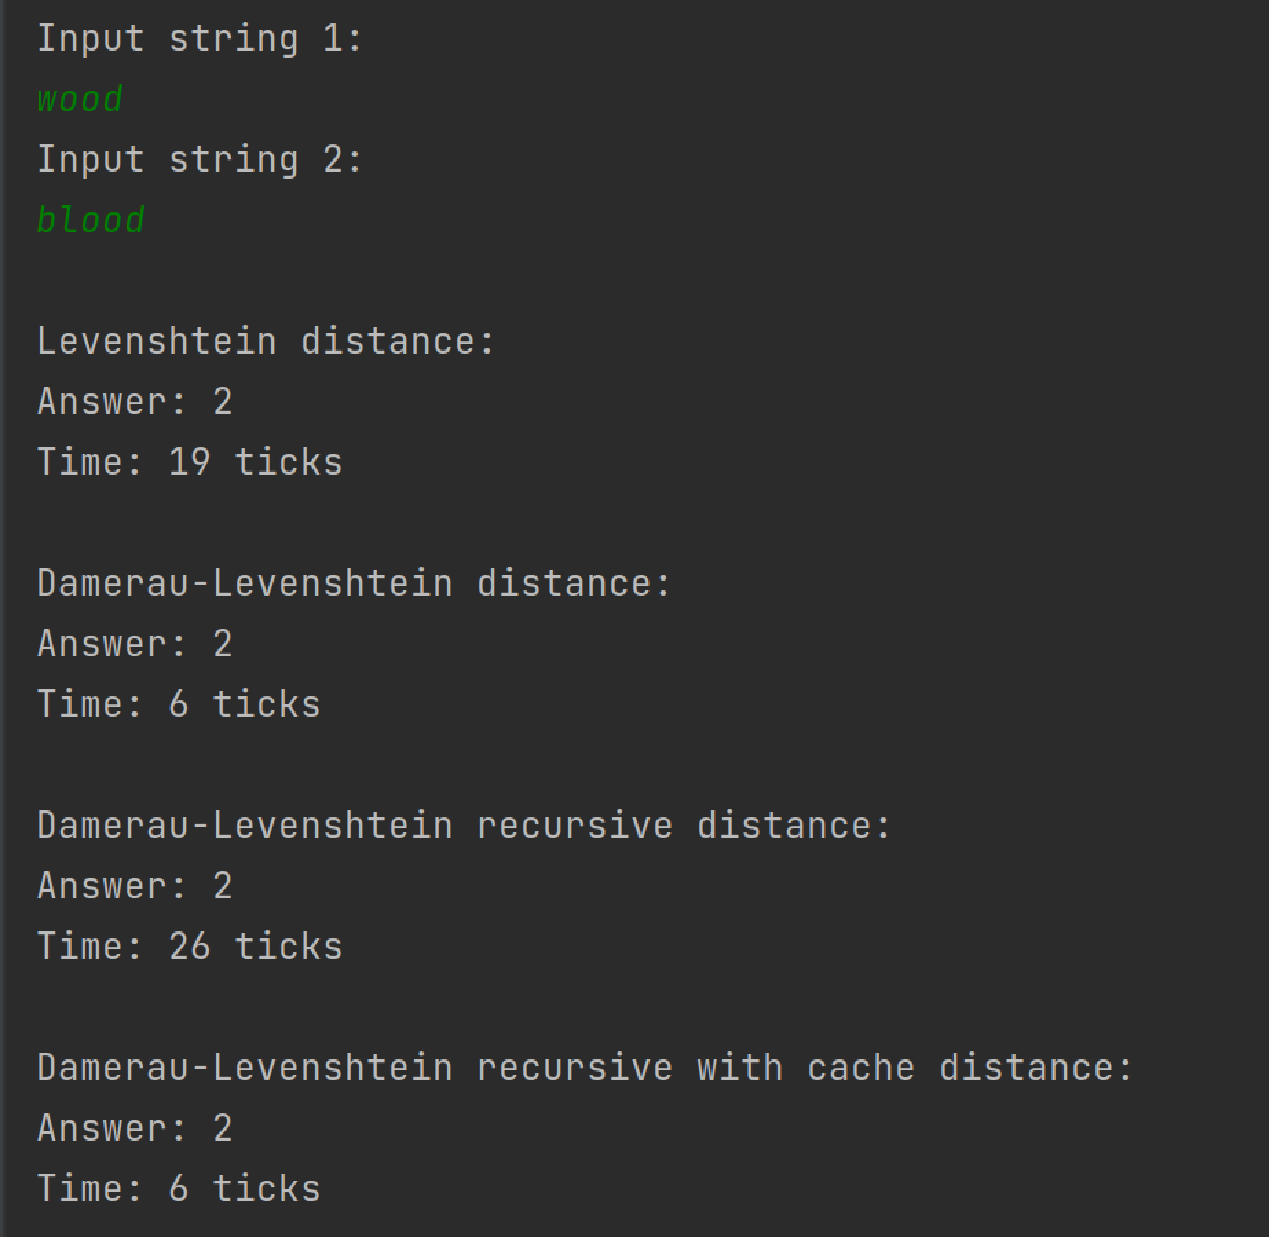
\includegraphics[width=0.6\linewidth]{include/example.pdf}
		\captionof{figure}{Пример работы программы}
		\label{img:example}
	\end{tabular}
\end{table}
\clearpage

\section{Измерение процессорного времени выполнения реализаций алгоритмов}

Время работы реализации алгоритмов было замерено с помощью функции clock. Полученное время измеряется в тиках, было замерено на компьютере подключенному к сети.

Результаты замеров в тиках приведены в таблице \ref{tbl:table}. В данной таблице для
значений, для которых тестирование не выполнялось, в поле результата
находится NaN.


\begin{table} [H]
	\caption{Таблица времени выполнения алгоритмов}
	\label{tbl:table}
	\begin{center}
		\begin{tabular}{|c|c|c|c|c|} 
		 	\hline
			\specialcell{Длина\\строк} & Левенштейн & Дамерау & Рекурсивный & \specialcell{Рекурсивный\\ с кэшем}\\  
		 	\hline
            1 & 0 & 0 & 0 & 0\\ \hline
            2 & 0 & 0 & 0 & 0\\ \hline
            3 & 0 & 0 & 0 & 0\\ \hline
            4 & 0 & 0 & 2 & 0\\ \hline
            5 & 0 & 1 & 11 & 0\\ \hline
            6 & 0 & 1 & 60 & 1\\ \hline
            7 & 1 & 2 & 327 & 1\\ \hline
            8 & 1 & 2 & 1786 & 1\\ \hline
            9 & 1 & 3 & 9840 & 2\\ \hline
            10 & 1 & 2 & NaN & 2\\ \hline
            11 & 1 & 2 & NaN & 2\\ \hline
            12 & 2 & 3 & NaN & 3\\ \hline
            13 & 2 & 3 & NaN & 3\\ \hline
            14 & 2 & 4 & NaN & 4\\ \hline
            15 & 3 & 4 & NaN & 5\\ \hline
            16 & 3 & 5 & NaN & 5\\ \hline
            17 & 3 & 5 & NaN & 6\\ \hline
            18 & 4 & 6 & NaN & 7\\ \hline
            19 & 4 & 7 & NaN & 8\\ \hline
            20 & 5 & 7 & NaN & 8\\ \hline
            25 & 7 & 11 & NaN & 13\\ \hline
            30 & 10 & 16 & NaN & 19\\ \hline
            35 & 14 & 21 & NaN & 27\\ \hline
            40 & 19 & 28 & NaN & 36\\ \hline
            45 & 23 & 35 & NaN & 45\\ \hline
            50 & 28 & 43 & NaN & 56\\ \hline
            60 & 40 & 61 & NaN & 81\\ \hline
            70 & 55 & 83 & NaN & 115\\ \hline
            80 & 71 & 107 & NaN & 151\\ \hline
            90 & 93 & 133 & NaN & 192\\ \hline
            100 & 119 & 66 & NaN & 237\\ \hline
		\end{tabular}
	\end{center}
\end{table}

На рисунке \ref{img:test4} представлена зависимость времени обработки строк от размеров строки для всех 4 реализованных алгоритмов. Замеры времени для реализации
рекурсивного алгоритма поиска расстояния Дамерау -- Левенштейна проводились до длины строк 9, так как его функция очень быстро растет.  
На рисунке \ref{img:test} приведены графики без рекурсивного алгоритма Дамерау -- Левенштейна, но на более длинных строчках.

\begin{table}[H]
	\centering
	\begin{tabular}{p{1\linewidth}}
		\centering
		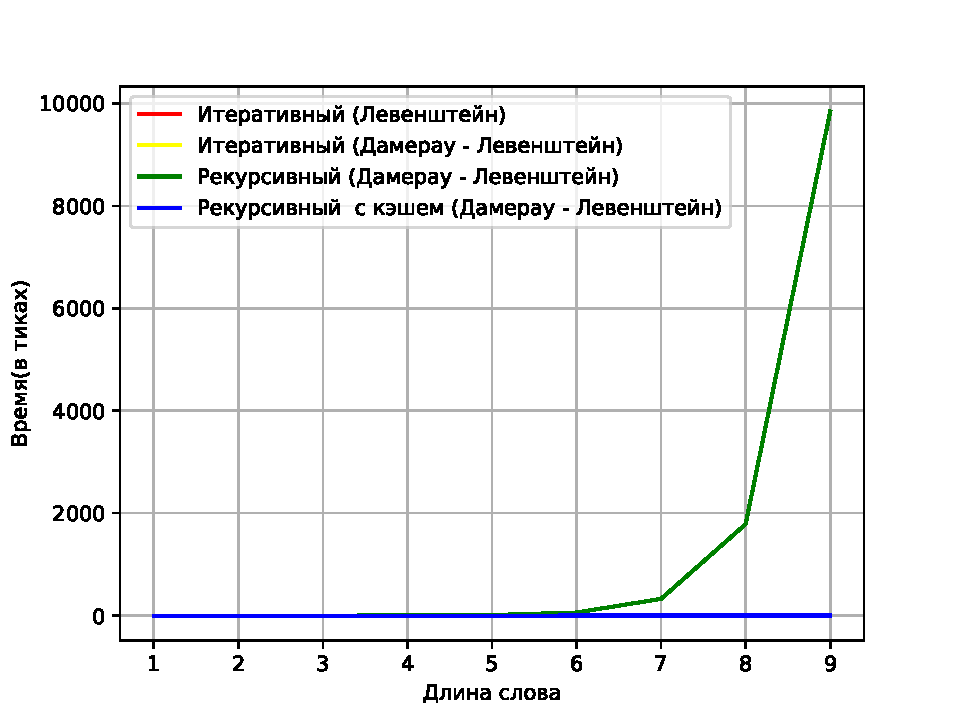
\includegraphics[width=0.8\linewidth]{include/test4.pdf}
		\captionof{figure}{Зависимость времени работы реализаций алгоритмов от размера строк для алгоритмов Левенштейна, нерекурсивного Дамерау -- Левенштейна, рекурсивного Дамерау -- Левенштейна, рекурсивного с кэшированием Дамерау -- Левенштейна}
		\label{img:test4}
	\end{tabular}
\end{table}

\begin{table}[H]
	\centering
	\begin{tabular}{p{1\linewidth}}
		\centering
		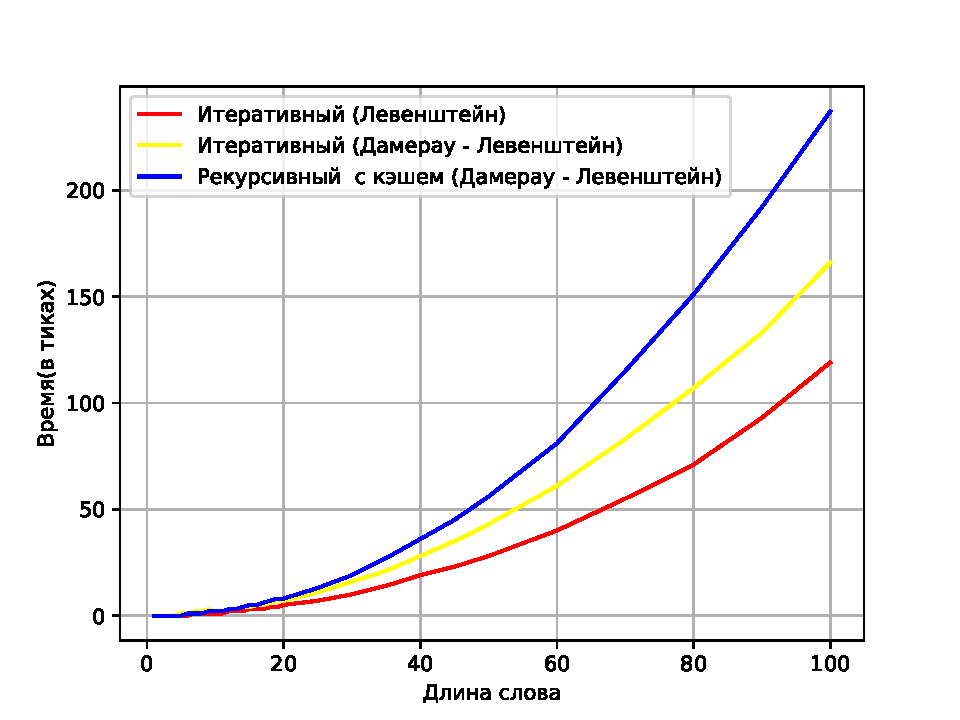
\includegraphics[width=0.8\linewidth]{include/test.pdf}
		\captionof{figure}{Зависимость времени работы реализаций алгоритмов от размера строк для алгоритмов Левенштейна, нерекурсивного Дамерау -- Левенштейна, рекурсивного с кэшированием Дамерау -- Левенштейна}
		\label{img:test}
	\end{tabular}
\end{table}


\section{Использование памяти}

Рассмотрим разницу рекурсивной и матричной реализаций алгоритмов
нахождения расстояния Дамерау -- Левенштейна.
Пусть длина строки $S_1$ -- n, длина строки $S_2$ -- m, тогда затраты памяти
на приведенные выше алгоритмы будут следующими:

\begin{enumerate}[label={\arabic*)}]
    \item Нерекурсивная реализация алгоритма поиска расстояния Левенштейна:
    \begin{itemize}
        \item строки $S_1, S_2$ занимают $(n + m) * sizeof(char)$;
        \item длины строк $S_1, S_2$ занимают $2 * sizeof(int)$;
        \item матрица занимает $(m + 1) * (n + 1) * sizeof(int)$;
        \item вспомогательные переменные занимают $sizeof(int) + sizeof(bool)$.
    \end{itemize}
    Всего: $(n + m) * sizeof(char) + sizeof(bool) + sizeof(int) * (3 + (m + 1) * (n + 1) )$ 
    \item Нерекурсивная реализация алгоритма поиска расстояния Дамерау -- Левенштейна:
    \begin{itemize}
        \item строки $S_1, S_2$ занимают $(n + m) * sizeof(char)$;
        \item длины строк $S_1, S_2$ занимают $2 * sizeof(int)$;
        \item матрица занимает $(m + 1) * (n + 1) * sizeof(int)$;
        \item вспомогательные переменные занимают $sizeof(int) + sizeof(bool)$.
    \end{itemize}
    Всего: $(n + m) * sizeof(char) + sizeof(bool) + sizeof(int) * (3 + (m + 1) * (n + 1) )$ 
    \item Рекурсивная реализация алгоритма поиска расстояния Дамерау -- Левенштейна (для каждого вызова):
     \begin{itemize}
        \item строки $S_1, S_2$ занимают $(n + m) * sizeof(char)$;
        \item длины строк $S_1, S_2$ занимают $2 * sizeof(int)$;
        \item вспомогательные переменные занимают $sizeof(int) + sizeof(bool)$;
        \item адрес возврата -- $sizeof(int*)$.
       
    \end{itemize}
   Для каждого вывода: $(n + m) * sizeof(char) + sizeof(bool) + sizeof(int*) + 3 * sizeof(int)$.
   
    Всего: $(n + m) *((n + m) * sizeof(char) + sizeof(bool) + sizeof(int*) + 3 * sizeof(int))$. 
    
    \item Рекурсивная с кешированием реализация алгоритма поиска расстояния Дамерау -- Левенштейна (для каждого вызова):
    
         \begin{itemize}
        \item строки $S_1, S_2$ занимают $(n + m) * sizeof(char)$;
        \item длины строк $S_1, S_2$ занимают $2 * sizeof(int)$;
        \item ссылка на матрицу -- $sizeof(int*)$;
        \item вспомогательные переменные занимают $5 * sizeof(int)$.
        \item адрес возврата -- $sizeof(int*)$.
    \end{itemize}
   Для каждого вывода: $(n + m) * sizeof(char) + 2 * sizeof(int*) + 7 * sizeof(int)$.
   
   Для всех вызовов память для хранения самой матрицы -- $(n + 1) *(m + 1) * sizeof(int)$.
   
    Всего: $(n + m) *((n + m) * sizeof(char) + 2 * sizeof(int*) + 7 * sizeof(int)) + (n + 1) *(m + 1) * sizeof(int)$ 
    
   
\end{enumerate}

